\subsection{Generalized Pruning Algorithm} \label{sec:GenPrun}

\begin{figure}
  \begin{subfigure}[t]{0.42\textwidth}
  \centering
  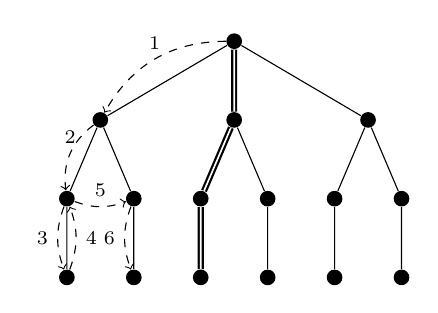
\begin{tikzpicture}[
    state/.style={circle, fill=black, inner sep=2pt},
    level distance=1.0cm,
    level/.style={sibling distance=17mm/#1}
]
\node [state] (a) {}
    child {node [state](b) {}
        child {node [state](c) {}
            child {node [state](d) {}}
            }
            child {node [state] (e) {}
            child {node [state] (f) {}}
            }
    }
    child {node [state](b1) {}
        child {node [state](b2) {}
            %child {node [state] {}}
            child {node [state](b3) {}}
            }
            child {node [state] {}
            child {node [state] {}}
            }
    }
    child {node [state] {}
        child {node [state] {}
            child {node [state] {}}
            }
            child {node [state] {}
            child {node [state] {}}
            }
    };
    \draw[->, dashed] (a) to [bend right=30] node [midway, above] {\scriptsize $1$} (b);
    \draw[->, dashed] (b) to [bend right=30] node [midway, above] {\scriptsize $2$} (c);
    \draw[->, dashed] (c) to [bend right=20] node [midway, left] {\scriptsize $3$} (d);
    \draw[->, dashed] (d) to [bend left=-20] node [midway, right] {\scriptsize $4$} (c);
    \draw[->, dashed] (c) to [bend right=20] node [midway, above] {\scriptsize $5$} (e);
    \draw[->, dashed] (e) to [bend right=20] node [midway, left] {\scriptsize $6$} (f);

    \draw[thick, double] (a) -- (b1);
    \draw[thick, double] (b1) -- (b2);
    \draw[thick, double] (b2) -- (b3);
\end{tikzpicture}%
\caption{\scriptsize Enumeration tree of the Lindner-Peikert algorithm for $3$-dimensional lattice with $\dvec = (3, 2, 1)$. }
\label{fig:TwoTreesLP}
\end{subfigure}
\hspace{10pt}
\begin{subfigure}[t]{0.47\textwidth}
\centering
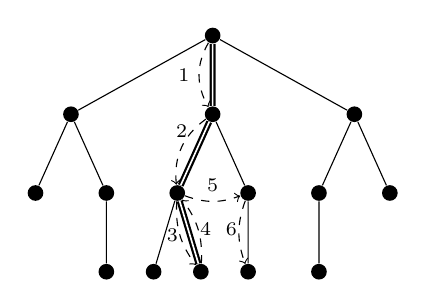
\begin{tikzpicture}[
    state/.style={circle, fill=black, inner sep=2pt},
    level distance=1.0cm,
    level/.style={sibling distance=18mm/#1}
]
\node [state] (a) {}
    child {node [state](b) {}
    	child {node [state] {} }
        child {node [state](c) {}
            child {node [state](d) {}}
            }
    }
    child {node [state](b1) {}
        child {node [state](b2) {}
            child {node [state] {}}
            child {node [state](b3) {}}
            }
            child {node [state](j) {}
            child {node [state](h) {}}
            }
    }
    child {node [state] {}
        child {node [state] {}
            child {node [state] {}}
            }
        child {node [state] {}}
    };
    \draw[->, dashed] (a) to [bend right=30] node [midway, left] {\scriptsize $1$} (b1);
    \draw[->, dashed] (b1) to [bend right=30] node [midway, above] {\scriptsize $2$} (b2);
    \draw[->, dashed] (b2) to [bend right=20] node [left, xshift=1mm] {\scriptsize $3$} (b3);
    \draw[->, dashed] (b3) to [bend left=-20] node [right, xshift=-1mm] {\scriptsize $4$} (b2);
    \draw[->, dashed] (b2) to [bend right=20] node [midway, above] {\scriptsize $5$} (j);
    \draw[->, dashed] (j) to [bend right=20] node [left, yshift=.4mm, xshift=1mm] {\scriptsize $6$} (h);

    \draw[thick, double] (a) -- (b1);
    \draw[thick, double] (b1) -- (b2);
    \draw[thick, double] (b2) -- (b3);
\end{tikzpicture}
\caption{\scriptsize Enumeration tree of the Generalized Pruning algorithm realized via some bounding function $\B$. As opposed to the left figure, the number of children varies for nodes on the same level.}
\label{fig:TwoTreesPrun}
\end{subfigure}
    \caption[Enumeration trees]{\footnotesize Enumeration tree of the Lindner-Peikert Algorithm (left) and the Generalized Pruning (right). The roots correspond to the initial call, the leaves contain the candidate error-vectors and the corresponding lattice vectors. The double-line represents the path (i.e.\ the choices of hyperplanes) that would have been chosen by the Babai's $\NP$ Alg.~\ref{alg:Babai}. The dashed curved arrows show the order of tree-traversals. On the left, the left-most child is visited first (usual depth-first tree-traversal). On the right, the `best' (w.r.t.\ the error-length)  child is chosen first (the \emph{best-first} traversal). 
    }
\label{fig:EnumTrees}
\end{figure}

\paragraph{Spherical and Linear-Length Pruning.} 

Note that the error-vector $\evec' = \sum_i e_i' \frac{\wbvec_i}{ \| \wbvec_i \|}$ is not explicitly bounded during the Lindner-Peikert's enumeration. 
It is done implicitly via restricting its individual coordinates $e_i'$. Each coordinate $e_i'$ is obtained by going one level down the enumeration tree: on level $k$ we compute $\evec'^{(k)} = \sum_{i=k+1}^m e_i' \frac{\wbvec_i}{ \| \wbvec_i \|}$ by adding $e'_{k+1}\frac{\wbvec_i}{ \| \wbvec_i \|}$ to $\evec'^{(k+1)}$ for an appropriately chosen coordinate $e'_{k+1}$ (see line \ref{algline:LPComputeError} in Alg.~\ref{alg:LP}).
By the end of the enumeration, $\evec'^{(k)}$ builds a final output $\evec'$ and hence, this final $\evec'$ will have length greater than $\| \evec'^{(k)} \|$. 
A moment's thought reveals that it is reasonable to make the number of children for a node dependent on the length of the error $\| \evec'^{(k)} \|$ associated to this node: the smaller this length is, the more children we want this node to have as it is more likely to lead to the correct solution, while if $\| \evec'^{(k)} \| \gg \sqrt{m} \alpha q$ (i.e.\ the accumulated error-length exceeds the expected length of the \LWE error), we might as well choose no children at all and stop the recursion for this node. This is why we use the term `pruning' as we prune the enumeration tree at some unpromising nodes.

For example, the \emph{Spherical Pruning} (\cite{SchE94}) chooses the number of the children for a $k\th$-level node with $\|\evec'^{(k)} \|^2 = \sum_{i=k+1}^m e_i'^2$ as $\TLandau  \left( \frac{1}{\| \wbvec_k \|^2} ( m (\alpha q)^2 - \sum_{i=k+1}^m e_i'^2) \right)$. This choice exactly captures our intuition: the shorter the accumulated error, the more children a node is allowed to have. We divide by $ \| \wbvec_k \|^2$ to get the actual number of the hyperplanes we recurse on (i.e.\ the number of children). It is easy to see that a pruning strategy enumerates all possible error-vectors that lie within the ball $\Ball(\tvec, \alpha q)$. 

Another pruning strategy, the \emph{Linear-Length Pruning} (\cite{EC:GamNguReg10}), reduces the search space of the Spherical Pruning by allowing a $k\th$-level error-vector to have norm $\| \evec'^{(k)} \|^2 \leq \TLandau( (m-k+1) (\alpha q)^2)$. This upper bound is the expected length of an $(m-k+1)$-dimensional vector with Gaussian entries of width $\alpha q$. It results, as in case of the Spherical Pruning, in the output error-vectors having norm $\TLandau(m \sqrt{\alpha q})$, but it is more restrictive on the intermediate levels.

There are several other pruning strategies considered in \cite{EC:GamNguReg10}, all aiming at reducing the search space by pruning the enumeration tree more aggressively, thus reducing the running time but sacrificing success probability (and hence, they are called \emph{Extreme Pruning} with the most `extreme' case being Babai's $\NP$). 
\vspace{10pt} %
\paragraph{Generalized Pruning.} All the enumeration strategies considered here can be described via a family of bounding functions $\B^{(k)}: \Q_{\geq 0}^{m-k} \rightarrow \Q_{\geq 0}$, $1 \leq k \leq m$. In general, this function may not even be efficiently computable in practice. For example, Aono in \cite{Ao14} suggests a way to find an optimal $\B^{(k)}$ given the Gram-Schmidt basis $\wBMat$ via solving an $m$-dimensional optimization problem. But for our $\GenPrun$ algorithm (Alg.~\ref{alg:GenPrun}) and its analysis we assume an efficiently computable family $\B^{(k)}$ which is given as an additional input.

%
% Generalized Pruning
%
\begin{algorithm}[t]
\caption{Generalized Pruning Algorithm $\GenPrun(\BMat, \protect \xvec, \protect \tvec, \protect \evec', \B^{(k)})$}
\label{alg:GenPrun}
\textbf{Input:} $\BMat=(\bvec_1, \ldots, \bvec_m) \in \Z^{m \times m}, \xvec\in\Q^m, \tvec \in \xvec+\Span(\BMat), \evec'\in\Q^m, \B^{(k)}$ \hfill ($\evec'=\xvec=0$ in the initial call)\\
\textbf{Output:} A set of pairs $(\vvec,\evec')$ with $\vvec\in \xvec+\Lat(\BMat)$ and $\evec' = \tvec-\vvec$ corresponding error vector
%\vspace{8pt}
\begin{algorithmic}[1]
\State $\xvec^{(k)}\gets \xvec, \tvec^{(k)}\gets \tvec,\evec'^{(k)}\gets\evec'$ 
\State Let $\wBMat\gets\GSO(\BMat)$
\If {$k=0$} \Return $\{(\xvec,\evec')\}$ \EndIf
\State Compute $c^{(k)}_1 \gets \bigScProd{\tvec^{(k)}}{\frac{\wbvec_k}{ \vphantom{\scalebox{1.6}x^2} \|\wbvec_k \|^2  }}$
\State
Let $e'_i = \ScProd{\evec'^{(k)}}{\frac{\wbvec_i}{\vphantom{\scalebox{1.6}x^2} \|\wbvec_i\|}}$ for $k< i \le m$ \Comment Coefficients of $\evec'$
\State Let $\Dmax^2 = \B^{(k)}(e'^2_m,\ldots,e'^2_{k+1})$ \Comment bound on distance of next hyperplanes \label{algline:GenPrunDmax}
\State Compute $c^{(k)}_j = \bigScProd{\xvec^{(k)}}{\frac{\wbvec_k}{\|{\wbvec_k}\|^2}} + i^{(k)}_j$ for all $i^{(k)}_j \in \Z$ s.t.\
$\abs{c_1^{(k)} - c_j^{(k)}}^2 \cdot \|\wbvec_k \|^2 \leq \Dmax^2$ \label{algline:GenPrunChoosePlane}
\For {\textbf{each} $(i^{(k)}_j, c^{(k)}_j)$} 
		\State $\xvec^{(k-1)}_j \gets \xvec^{(k)}+i^{(k)}_j \bvec_k$ \label{algline:GenPrunChooseTranslate}
		\Comment $U_j^{(k-1)} = \xvec^{(k-1)}_j+\Lat(\BMat^{(k-1)})$ are the nearby planes
		\State $\evec'^{(k-1)}_j \gets \evec'^{(k)} + (c^{(k)}_1-c^{(k)}_j)\wbvec_k$
		\State $\tvec^{(k-1)}_j =\tvec^{(k)} - (c^{(k)}_1-c^{(k)}_j)\wbvec_k$ \Comment Project onto $U_j^{(k-1)}$ 
\State \Return $\bigcup_j \GenPrun ((\bvec_1,\ldots,\bvec_{k-1}), \xvec^{(k-1)}_j,\tvec^{(k-1)}_j,\evec'^{(k-1)}_j, \B^{(k)})$
\EndFor
\end{algorithmic} 
\end{algorithm}

The algorithm computes the maximal allowed distance (denoted $\Dmax$) to the next hyperplanes (line \ref{algline:GenPrunDmax} of Alg.~\ref{alg:GenPrun}) and chooses only the hyperplanes for which $e'^2_k$ satisfies $e'^2_k < \B^{(k)} (e'^2_m, \ldots, e'^2_{k+1}) = \Dmax^2$. The search region of \GenPrun is
\begin{equation*} 
	V_{\GP} = \Bigl\{ \evec' = \sum_k e'_k \frac{\wbvec_k }{\| \wbvec_k \| } \colon e_k^2 \leq \B^{(k)}(e'^2_m, \ldots, e'^2_{k+1}) \; \forall k \Bigr\}.	
\end{equation*}

The algorithm successfully solves the \LWE problem if the \LWE error-vector $\evec$ is contained in the search region $V_{\GP}$. It is easy to see that Generalized Pruning captures all the enumeration strategies discussed here. Namely,

\begin{itemize}
	\item $\B^{(k)}(e'^2_m, \ldots, e'^2_{k+1}) = \left( \frac{\| \wbvec_k \|}{2} \right)^2 $: Babai's $\NP$
	\item $\B^{(k)}(e'^2_m, \ldots, e'^2_{k+1}) = \left( \frac{d_k \| \wbvec_k \|}{2} \right)^2 $: Lindner-Peikert's $\NPs$
	\item $\B^{(k)}(e'^2_m, \ldots, e'^2_{k+1}) = \TLandau(m (\alpha q)^2) - \sum_{i=k+1}^m e'^2_i$: Spherical Pruning
	\item $\B^{(k)}(e'^2_m, \ldots, e'^2_{k+1}) = \TLandau( (m-k)(\alpha q)^2) - \sum_{i=k+1}^m e'^2_i $: Linear Pruning
	\item $\B^{(k)}(e'^2_m, \ldots, e'^2_{k+1}) = R_k^2 -  \sum_{i=k+1}^m e'^2_i$: pruned strategy with some level-dependent bounds $R_k$.  
\end{itemize}
 
All the extreme pruning approaches of \cite{EC:GamNguReg10} as well any numerically optimized strategy are covered by the last choice of $\B^{(k)}$.

For the analysis, we extend $\B^{(k)}$ to real-valued arguments so that we can apply the algorithm to a continuous Gaussian.

\paragraph{Analysis.} As before, we are interested in the ratio $\rho(\GP) = \frac{T(\GP)}{\Psucc(\GP)}$ ($\GP$ is used as a shorthand for Generalized Pruning). A family of bounding functions $\B^{(k)}$ defines the search region on level $k$ as
\begin{equation}\label{eq:VGP}
	V_{\GP}(k) =  \Bigl\{ \evec' = \sum_{i=k+1}^m e'_i \frac{\wbvec_i }{\| \wbvec_i \| } \colon e_j^2 \leq \B^{(j)}(e'^2_m, \ldots, e'^2_{j+1}) \;  k < j \leq m \Bigr\}.
\end{equation}

Let $N_k$ be the number of nodes at level $k$ and $p_k$ be the probability that the correct solution is retained on level $k$ (i.e.\ there exists a node with $\evec^{(k)}$ that can be extended to the correct \LWE error $\evec$ by traversing the tree down to the last level). We define a \emph{reasonable pruning} via requiring a set of conditions to be met by $\B^{(k)}, N_k,  p_k$. We assume that the error we seek for, follows a continuous Gaussian with parameter $\alpha q$ and that $ \| \wbvec_m \| < \alpha q < \| \wbvec_1 \| $. The latter is satisfied by the choice of $\beta$.

\begin{definition}[Reasonable Pruning] \label{def:ReasonablePruning}
Let $k^*$ be the maximal level s.t.\ $\| \wbvec_{k^*} \| > \alpha q$. The Generalized Pruning algorithm with the associated $\B^{(k)}$ is \emph{reasonable} if the following conditions are satisfied
 \begin{enumerate}
 	\setlength\itemsep{0.1em}
 	\item $\B^{(k)}(e'^2_m, \ldots, e'^2_{k+1}) + \sum_{i=k+1}^m e'^2_i = \TLandau(m (\alpha q)^2)$ 
 	\item $\Psucc(\GP) \geq 2^{-\bigO(m)} \cdot p_{k^*}$
 	\item $N_k \leq 2^{\bigO(m)} \cdot N_{k^*}$ for $k \leq k^*$
 	\item $\frac{N_{k-1}}{N_k} = \WLandau(1)$ for $k \geq k^*$
 	\item $V_{\GP}(k^*)$ is convex.
 \end{enumerate}
\end{definition} 

Informally, the conditions in Def.~\ref{def:ReasonablePruning} have the following meaning: Condition 1 implies that we prune the nodes with the accumulated error larger than the expected length of the \LWE error. Conditions 2 and 3 mean that as soon as the correct error survived until the `critical' level $k^*$, we can find $\evec$ with high probability (Condition 2) at essentially no additional cost (Condition 3). For example, from $k^*$ down, we can start the Babai's $\NP$ algorithm. Condition 4 ensures that for levels above $k^*$ we choose \emph{at least} a constant number of hyperplanes (line \ref{algline:GenPrunChoosePlane} in Alg.~\ref{alg:GenPrun}) to recurse on. Note that on these upper levels we have $\| \wbvec_k \| < \alpha q$ for $k>k^*$, so we must have $\WLandau(1)$ hyperplanes at distance at most $\alpha q$.

We elaborate on the convexity condition a bit more. Let us take a closer look at the search region $V_{\GP}$. From the way the error-vectors $\evec'^{(k)}$ are constructed during the algorithm, the number of nodes at level $k$, denoted $N_k$, is the number of points in $V_{\GP}(k) - \evec$ that belong to the lattice $\Lat(\wbvec_m, \ldots, \wbvec_{k+1})$, i.e.\ to the orthogonal projection of $\Lat(\BMat)$ onto $\Span(\bvec_1, \ldots, \bvec_k)$ (the shift by $\evec$ does not change $N_k$ asymptotically but is needed for the proof below). The Gaussian Heuristic suggests that
\begin{equation*} %\label{eq:GaussHeuristic}
	N_k \approx \frac{\vol V_{\GP}(k)}{\prod_{i=k+1}^m \| \wbvec_i \|}.
\end{equation*}

We could use this approximation in our theorem below, but since it is enough in our setting to upper-bound $N_k$ up to a factor of $2^{\bigO(m)}$, we can prove the above equation by relying on a variant of Minkowski's Convex Body Theorem. 
Roughly, this theorem tells us that if an $m$-dimensional 0-symmetric convex point-set ($V_{\GP}(k)$ for us) has volume larger than the volume of a lattice, then it contains a non-zero point of this lattice. 

The generalization of this result is due to Rado \cite{R46}: instead of a 0-symmetric convex set, he considers a non-negative integrable function $f(\xvec)$  and connects the quantity $\sum_{\vvec \in \Lat} f(\vvec)$ with the value $\mathcal{V}(f) =~ \int_{- \infty < x_i < \infty} f(\xvec) \d \xvec$. The convexity condition of the set is replaced by the quasi-concavity condition for $f$: for a linear map ${\Lambda}$ from an $m$-dimensional vector space into itself, the function $f$ must satisfy $f(\Lambda \xvec - \Lambda \yvec) \geq \min \{ f(\xvec), f(\yvec) \}$.
Later in Thm.~\ref{thm:GenPrunRunTime}, we consider $\Lambda$ acting like $\Lambda \xvec = \tfrac{1}{2} \xvec$. 
Minkowski's Convex Body Theorem is a special case of the Thm.~\ref{thm:Rado} for $f(\xvec)$ being a characteristic function of a convex symmetric set $V$ in which case $\mathcal{V}(f) = \vol V$.

\begin{thm}[Rado's generalization of Minkowski's Convex Body Theorem] \label{thm:Rado}
Let $f(\xvec)$ be a non-negative integrable function with the property $f(\Lambda \xvec - \Lambda \yvec) \geq \min \{ f(\xvec), f(\yvec) \}$ for all $\xvec, \yvec \in \R^m$ and a linear map $\Lambda: \R^m \rightarrow \R^m$. Then
\begin{equation} \label{eq:RadosThm}
	f(\zerovec) + \tfrac{1}{2} \sum_{\zerovec \neq \vvec \in \Lat} f(\vvec) \geq \frac{\abs{\det \Lambda}}{\det (\Lat)} \mathcal{V}(f),
\end{equation}
for every lattice $\Lat$, where 
\[
\mathcal{V}(f) = \int\limits_{\substack{ - \infty < x_i < \infty \\ 1 \leq i \leq m }} f(\xvec) \d \xvec,
\] 
and $\det(\Lambda)$ is the determinant of the $m \times m$ matrix that defines the transformation $\Lambda$.
\end{thm}
Following the proof of the theorem (see the book of Cassels \cite[Chap.\ III]{Cas97} for a comprehensive proof) and setting $\Lambda \xvec = \tfrac{1}{2} \xvec$ (so $\abs{\det \Lambda} = 2^{-m}$), we observe that up to $2^{\bigO(m)}$ the inequality given in Eq.~\eqref{eq:RadosThm} is an equality, so in our proof we rely on the fact that
\begin{equation} \label{eq:RadoEq}
f(\zerovec) + \tfrac{1}{2} \sum_{\zerovec \neq \vvec \in \Lat} f(\vvec) = \frac{2^{\pm \bigO(m)}}{\det (\Lat)} \mathcal{V}(f).
\end{equation}

Now we have the tools to present the main theorem of this section \emph{without} relying on the Gaussian Heuristic. 
We apply Eq.~(\ref{eq:RadoEq}) to the function $f(\xvec) = \tfrac{1}{(\alpha q)^{k^*}} \int_{V_{\GP}(k^*)} \exp \left( \frac{-\pi \| \yvec \|^2}{(\alpha q)^2} \right) \d \yvec$ and to the lattice $\Lat(\wbvec_m, \ldots, \wbvec_{k^*+1})$, where $k^*$ is the `critical' level as in Def.~\ref{def:ReasonablePruning}. $f(\xvec)$ is the convolution of the Gaussian density function with the characteristic function of our convex search region $V_{\GP}(k^*)$ and hence, it satisfies the quasiconcavity condition of Thm.~\ref{thm:Rado}. 

\begin{thm}[Analysis of the $\GenPrun$ Algorithm~\ref{alg:GenPrun}] \label{thm:GenPrunRunTime}
Given a $\beta = \TLandau(n)$-\BKZ reduced basis that arises from $m = \TLandau(n)$ \LWE-samples with parameters $(n, q=\bigO(n^{\cq}), \alpha = \bigO(1 / n^{\ca}) )$ for positive constants $\cq >\ca$ s.t.\ $\frac{m}{2 \beta} + \frac{n}{m} \cq - \ca >0$, any reasonable (as in Def.~\ref{def:ReasonablePruning}) pruning algorithm $\GP$ has an expected (over the choice of $\evec$) running time/success probability trade-off
\[
	\rho(\GP) = \frac{\E[T(\GP)]}{\Psucc(\GP)} = 2^{\frac{1}{2} \bigl(\frac{m}{2\beta}-\ca + \frac{n}{m} \cq  \bigr)^2 (1+\smallo(1)) \cdot \beta\log\beta},
\]
with $\poly(m)$ memory (using depth-first search) assuming the Geometric Series Assumption holds and the \LWE error follows a continuous Gaussian distribution.
\end{thm}

\begin{proof}
	The amount of work done on one node of the enumeration tree of Alg.~\ref{alg:GenPrun} is clearly $\poly(m)$, so the total running time is $T(\GP) = \poly(m) \cdot \sum N_k$. For the `critical' level $k^*$ (i.e.\ maximal level with $\| \wbvec_{k^*} \| > \alpha q$), we have $N_i < 2^{\bigO(m)}$ for all $i$ (for $i<k^*$ due to Condition 3 in Def.~\ref{def:ReasonablePruning}, for $i>k^*$ by the definition of $N_k$). So for a reasonable pruning strategy, it holds that
	\[
		T(\GP) = 2^{\bigO(m)} N_{k^*}.
	\]
	As discussed above, $N_{k^*}$ is (up to $2^{\bigO(m)}$) the number of lattice vectors $\vvec \in \Lat (\wbvec_m, \ldots, \wbvec_{k^* +1})$ that lie in the convex region $V_{\GP} - \evec$. Taking the expectation over the choice of $\evec$, 
	\[
		\E_{\evec}[N_{k^*}] = \sum_{\vvec \in \Lat (\wbvec_m, \ldots, \wbvec_{k^* +1})} f(x) \qquad \text{where} \qquad f(\xvec) = \tfrac{1}{(\alpha q)^{k^*}} \int\limits_{V_{\GP}(k^*)} \exp \left( \frac{-\pi \| \yvec \|^2}{(\alpha q)^2} \right) \d \yvec.
	\]
	This expectation is essentially the left-hand side of Eq.~(\ref{eq:RadoEq}). Note that $f(x)$ is quasiconcave (as it is a convolution of two log-concave functions: the Gaussian density function and the characteristic function of the convex region $V_{\GP}$). For $\Lat = \Lat(\wbvec_m, \ldots, \wbvec_{k^* +1})$, we obtain
	\begin{align*}
			\E_{\evec}[N_{k^*}] &= \frac{2^{\pm \bigO(m)}}{\det (\Lat)} \int f(\xvec) \d \xvec = 
			\frac{2^{\pm \bigO(m)}}{\det (\Lat)} \int\limits_{V_{\GP}(k^*)} \int\limits_{\substack{ - \infty < y_i < \infty \\ 1 \leq i \leq m }} \frac{1}{(\alpha q)^{k^*}} \exp \left( \frac{-\pi \| \yvec \|^2}{(\alpha q)^2} \right) \d \yvec \d \xvec =  \\
			&= \frac{2^{\pm \bigO(m)} \vol V_{\GP}(k^*)}{\det (\Lat)}.  
	\end{align*}
	If the pruning is reasonable, we have $\Psucc(\GP) = 2^{-\bigO(m)} \cdot p_{k^*}$, where $p_{k^*}$ is the probability that there exist a vector in $V_{k^*}$ s.t.\ its $m-k^*$ coordinates extend to the \LWE error-vector, yielding
	\begin{align*}
		\frac{\E[T(\GP)]}{\Psucc(\GP)} &= \frac{2^{\pm \bigO(m)} \vol V_{\GP}(k^*)}{\det (\Lat) \cdot \tfrac{1}{(\alpha q)^{m-k^*}} \int\limits_{\xvec \in V_{\GP}(k^*)} \exp(- \tfrac{\pi \| \xvec \|^2}{(\alpha q)^2}) \d \xvec} = 
		\frac{2^{\pm \bigO(m)} \cdot (\alpha q)^{m-k^*} \vol V_{\GP}(k^*) }{\prod_{i=m-k^*}^m \| \wbvec_i \| \cdot \int\limits_{\xvec \in V_{\GP}(k^*)} \exp(- \tfrac{\pi \| \xvec \|^2}{(\alpha q)^2})} = \\
		&= \frac{2^{\pm \bigO(m)} \cdot (\alpha q)^{m-k^*} \int_{\xvec \in V_{\GP}(k^*)} 1 \d \xvec}{\prod_{i=m-k^*}^m \| \wbvec_i \| \cdot \int_{\xvec \in V_{\GP}(k^*)} 1 \d \xvec} = 
		2^{\frac{1}{2} \bigl(\frac{m}{2\beta}-\ca + \frac{n}{m} \cq  \bigr)^2 (1+\smallo(1)) \cdot \beta\log\beta},
	\end{align*} 
	where for the third equality we used Condition 1 in Def.~\ref{def:ReasonablePruning} stating that $e^{-\bigO(m)} \leq \exp(- \tfrac{\pi \| \xvec \|^2}{(\alpha q)^2}) \leq 1$ for any $\xvec \in V_{\GP}(k^*)$.
\end{proof}

We remark that for a pruning strategy that has $\Psucc \leq p_{k^*}$ and $T \geq \poly(m) N_{k^*}$, the result of Thm.~\ref{thm:GenPrunRunTime} gives a lower bound on the trade-off $\rho$ for such a strategy. 

Finally, note that the Lindner-Peikert $\NPs$ algorithm is a corner-case of a reasonable pruning: in the corners of the parallelepiped-shaped search region $V_{\NPs}$ Condition 1 is not satisfied. This is why we analyzed it separately. Now we can move on to the discussion on the total complexity of the \BDD attack on \LWE where we balance the running time of the reduction and enumeration phases.